\documentclass[10pt,twocolumn]{article}
% Shared two-column preamble for the three research papers.
% Use with: \documentclass[10pt,twocolumn]{article}
% Then in main.tex: % Shared two-column preamble for the three research papers.
% Use with: \documentclass[10pt,twocolumn]{article}
% Then in main.tex: % Shared two-column preamble for the three research papers.
% Use with: \documentclass[10pt,twocolumn]{article}
% Then in main.tex: \input{../../shared/latex/twocolumn_preamble.tex}

\usepackage[margin=0.75in]{geometry}
\usepackage[utf8]{inputenc}
\usepackage[T1]{fontenc}
\usepackage{lmodern}
\usepackage{microtype}
\usepackage{amsmath,amssymb,amsthm}
\usepackage{graphicx}
\usepackage{booktabs}
\usepackage{caption}
\usepackage{subcaption}
\usepackage{hyperref}
\usepackage{url}
\usepackage{xcolor}
\usepackage{algorithm}
\usepackage{algorithmic}
\usepackage{multirow}
\usepackage{titlesec}
\usepackage{authblk}

\hypersetup{colorlinks=true,linkcolor=blue!50!black,citecolor=blue!50!black,urlcolor=blue!50!black}

\titleformat{\section}{\normalfont\large\bfseries}{\thesection}{0.6em}{}
\titleformat{\subsection}{\normalfont\bfseries}{\thesubsection}{0.5em}{}

\captionsetup{font=small,labelfont=bf,skip=4pt}
\setlength{\columnsep}{0.25in}
\setlength{\parskip}{2pt}

\newtheorem{theorem}{Theorem}
\newtheorem{proposition}[theorem]{Proposition}
\newtheorem{definition}[theorem]{Definition}


\usepackage[margin=0.75in]{geometry}
\usepackage[utf8]{inputenc}
\usepackage[T1]{fontenc}
\usepackage{lmodern}
\usepackage{microtype}
\usepackage{amsmath,amssymb,amsthm}
\usepackage{graphicx}
\usepackage{booktabs}
\usepackage{caption}
\usepackage{subcaption}
\usepackage{hyperref}
\usepackage{url}
\usepackage{xcolor}
\usepackage{algorithm}
\usepackage{algorithmic}
\usepackage{multirow}
\usepackage{titlesec}
\usepackage{authblk}

\hypersetup{colorlinks=true,linkcolor=blue!50!black,citecolor=blue!50!black,urlcolor=blue!50!black}

\titleformat{\section}{\normalfont\large\bfseries}{\thesection}{0.6em}{}
\titleformat{\subsection}{\normalfont\bfseries}{\thesubsection}{0.5em}{}

\captionsetup{font=small,labelfont=bf,skip=4pt}
\setlength{\columnsep}{0.25in}
\setlength{\parskip}{2pt}

\newtheorem{theorem}{Theorem}
\newtheorem{proposition}[theorem]{Proposition}
\newtheorem{definition}[theorem]{Definition}


\usepackage[margin=0.75in]{geometry}
\usepackage[utf8]{inputenc}
\usepackage[T1]{fontenc}
\usepackage{lmodern}
\usepackage{microtype}
\usepackage{amsmath,amssymb,amsthm}
\usepackage{graphicx}
\usepackage{booktabs}
\usepackage{caption}
\usepackage{subcaption}
\usepackage{hyperref}
\usepackage{url}
\usepackage{xcolor}
\usepackage{algorithm}
\usepackage{algorithmic}
\usepackage{multirow}
\usepackage{titlesec}
\usepackage{authblk}

\hypersetup{colorlinks=true,linkcolor=blue!50!black,citecolor=blue!50!black,urlcolor=blue!50!black}

\titleformat{\section}{\normalfont\large\bfseries}{\thesection}{0.6em}{}
\titleformat{\subsection}{\normalfont\bfseries}{\thesubsection}{0.5em}{}

\captionsetup{font=small,labelfont=bf,skip=4pt}
\setlength{\columnsep}{0.25in}
\setlength{\parskip}{2pt}

\newtheorem{theorem}{Theorem}
\newtheorem{proposition}[theorem]{Proposition}
\newtheorem{definition}[theorem]{Definition}

\newcommand{\gptTwoIDmidShort}{8.61}
\newcommand{\gptTwoIDmidLong}{0.89}
\newcommand{\gptTwoAnisoMidShort}{0.523}
\newcommand{\gptTwoAnisoMidLong}{0.414}
\newcommand{\gptTwoEffRankDrop}{-267.56}
\newcommand{\gptTwoMaxCtx}{1024}
\newcommand{\gptTwoNumLayers}{12}


\title{Information Geometry and Embedding Collapse in Long-Context Transformers}
\author[1]{Luis Benvenuto}
\affil[1]{Independent Research}
\date{\today}

\begin{document}
\twocolumn[
\maketitle
\begin{@twocolumnfalse}
\begin{abstract}
\noindent We study how the geometry of contextual embeddings in autoregressive
language models deforms as the input context grows. Three complementary
diagnostics are proposed: a TwoNN-based intrinsic dimension, a pairwise
anisotropy measurement extending Ethayarajh~(2019), and a discrete curvature
proxy based on local PCA over $k$-nearest-neighbour patches. Applied to a
GPT-2 backbone on a long-document corpus across context lengths from
$128$ to $\gptTwoMaxCtx$ tokens, we observe a clean drop of intrinsic
dimension in the middle layers from $\gptTwoIDmidShort$ to $\gptTwoIDmidLong$
and an anisotropy shift from $\gptTwoAnisoMidShort$ to $\gptTwoAnisoMidLong$, with
effective rank decreasing monotonically. The pipeline is configuration-driven
and rescales to 7B-parameter open-weight models and $131{,}072$-token contexts
without code changes.
\end{abstract}
\vspace{1em}
\end{@twocolumnfalse}
]

\section{Introduction}

Long-context language models have become routine: Gemini 1.5, Claude, GPT-4,
and open-weight architectures such as Llama 3 routinely ingest tens of
thousands of tokens. The empirical observation that downstream quality often
degrades super-linearly with context length is widely reported but poorly
understood from a geometric standpoint. We ask a specific question:

\begin{quote}
\emph{Does the hidden-state manifold of a transformer language model undergo
a measurable phase transition as the context length grows, and if so, where
in the network does it occur?}
\end{quote}

A geometric account is attractive because it sits beneath the architectural
details. Whatever positional encoding, attention pattern, or rotary
modification is in use, the residual stream lives in $\mathbb{R}^d$ and
inherits a metric, a dimension, and a curvature. If long-context degradation
were primarily geometric---an attractor collapse of the residual stream
toward a low-dimensional subspace---we should be able to detect that collapse
without any reference to the task.

We make three contributions. \textbf{(i)} We define a triple of cheap, easily
implementable geometric diagnostics: an intrinsic dimension estimator
(TwoNN), a pairwise anisotropy measure, and a local-PCA curvature proxy.
\textbf{(ii)} We sweep these diagnostics over a four-decade range of context
lengths on GPT-2, releasing a reproducible pipeline that scales without code
changes to Llama-3-8B and Mistral-7B at $131{,}072$ tokens given GPU
resources. \textbf{(iii)} We show that, even on a small backbone, the
predicted collapse is visible: intrinsic dimension drops by roughly an order
of magnitude in the middle layers between short and long contexts, anisotropy
rises, and effective rank decreases monotonically.

The remainder of the paper is organised as follows. Section~\ref{sec:related}
reviews related work on anisotropy and intrinsic dimensionality. Section~\ref{sec:method}
formalises the diagnostics and Section~\ref{sec:experiments} the sweep.
Section~\ref{sec:results} reports findings, Section~\ref{sec:discussion}
interprets them, and Section~\ref{sec:conclusion} concludes.

\section{Related Work}\label{sec:related}

\paragraph{Anisotropy in contextual embeddings.} Ethayarajh~\cite{ethayarajh2019contextual}
showed that average pairwise cosine similarity between contextualised tokens
in BERT, GPT-2, and ELMo grows with depth, contradicting the implicit
assumption that contextual vectors live on a uniform unit sphere. Subsequent
work~\cite{cai2021isotropy,bis2021too} confirmed the phenomenon, attributed
it to a small number of dominant directions, and proposed whitening-based
corrections. Our anisotropy measurement is a direct extension of
Ethayarajh's, sampled across context lengths rather than across depths.

\paragraph{Intrinsic dimensionality of representations.} The TwoNN estimator
of Facco et al.~\cite{facco2017twonn} provides a non-parametric estimate of
the intrinsic dimension of a point cloud from the ratio of first and second
nearest-neighbour distances. It has been applied to image classifiers
\cite{ansuini2019id} and, more recently, to language models, where intrinsic
dimension has been argued to track generalisation and abstraction depth.
We adopt TwoNN because it is robust in the high-dimensional regime where
covariance-based estimators degenerate.

\paragraph{Long-context behaviour.} Several works~\cite{liu2024lost,xiong2024effective}
report systematic degradation of long-context accuracy. Most are
task-driven (question answering, needle-in-a-haystack). Our angle is
orthogonal: we instrument the residual stream geometrically and check
whether collapse precedes task failure.

\paragraph{Mechanistic interpretability.} Activation patching and circuit
discovery~\cite{wang2022interpret,nanda2023progress} are complementary
lenses. Where they ask \emph{which heads carry a computation}, we ask
\emph{what shape the representation has at all}. The two approaches share
a methodological commitment: study what is actually there, before
proposing remediation.

\section{Methodology}\label{sec:method}

\subsection{Setup}
Let $f_\theta$ be a decoder-only transformer with $L$ layers and hidden
dimension $d$. For input $x \in V^*$, denote by $h^{(\ell)}_i(x) \in
\mathbb{R}^d$ the residual-stream activation at layer $\ell$ and position $i$.
Given a context length $T$, we sample documents from a corpus, truncate to
$T$ tokens, and assemble a point cloud
\[
\mathcal{X}^{(\ell)}_T \;=\; \{\, h^{(\ell)}_i(x) \,\mid\, x \in \mathcal{D},\, 1\le i \le T \,\}\subset \mathbb{R}^d.
\]
We then compute three diagnostics on each cloud.

\subsection{Intrinsic dimension (TwoNN)}
For each point $p \in \mathcal{X}$ let $r_1(p), r_2(p)$ be its first- and
second-nearest-neighbour distances. Facco et al.\ show that
$\mu(p) := r_2(p)/r_1(p)$ follows a Pareto distribution with parameter $d$,
yielding the maximum-likelihood estimator
\begin{equation}
\hat{d}_{\mathrm{TwoNN}} = \frac{N}{\sum_{p} \log\mu(p)},
\label{eq:twonn}
\end{equation}
where $N$ is the number of valid samples. We truncate the upper tail at the
$90$th percentile of $\mu$ to suppress boundary effects.

\subsection{Anisotropy}
Following~\cite{ethayarajh2019contextual}, we draw $M$ random index pairs
$(i,j)$ uniformly without replacement and define
\begin{equation}
A(\mathcal{X}) = \frac{1}{M}\sum_{(i,j)}\frac{\langle x_i, x_j\rangle}{\lVert x_i\rVert\,\lVert x_j\rVert}.
\label{eq:aniso}
\end{equation}
A spherically uniform cloud satisfies $A \approx 0$; $A$ close to $1$
indicates collapse onto a narrow cone.

\subsection{Local-PCA curvature proxy}
For a subsample of $S \le N$ anchor points, retrieve the $k$ nearest
neighbours, centre them, and compute singular values
$\sigma_1 \ge \dots \ge \sigma_k$. Let
\begin{equation}
C(p) = \frac{\sum_{j>m}\sigma_j^2}{\sum_{j\le m}\sigma_j^2 + \varepsilon},
\label{eq:curv}
\end{equation}
where $m$ is the count of \emph{leading} directions (we use $m=3$). A flat
manifold concentrates mass in the leading directions ($C\to 0$); a
high-curvature region spreads mass across all directions ($C$ large).
We report $\overline{C} = \mathbb{E}_p[C(p)]$.

\subsection{Effective rank}
For completeness we report the effective rank of the centred activation
covariance, $\exp\!\big({-\sum_i p_i\log p_i}\big)$, where $p_i = \sigma_i/\sum_j\sigma_j$.
This gives a smooth, dimensionless measure of how many directions carry
appreciable variance and complements the discrete TwoNN estimate.

\section{Experiments}\label{sec:experiments}

\paragraph{Models.} The local pipeline uses GPT-2 small ($\gptTwoNumLayers$
blocks, hidden $d=768$); the GPU configuration (\texttt{configs/gpu\_full.yaml})
switches to Llama-3-8B and Mistral-7B without code changes.

\paragraph{Corpus.} For reproducibility on commodity hardware we use a
self-contained ArXiv-style abstract corpus (eight long documents,
concatenated to reach the target context length). The GPU configuration
streams ArXiv summarisation data via Hugging Face datasets.

\paragraph{Context-length sweep.} We sweep $T \in \{128, 256, 512, \gptTwoMaxCtx\}$
on the local configuration; the GPU configuration extends the sweep to
$131{,}072$ tokens. For each $T$ and each layer $\ell$, all metrics are
computed on a subsample of up to $4000$ tokens to bound running time.

\paragraph{Hyperparameters.} TwoNN uses the $90$th-percentile truncation
recommended by Facco et al. Anisotropy uses $M=2000$ random pairs.
Curvature uses $k=20$ neighbours, $m=3$ leading directions, and $S=512$
anchors.

\paragraph{Implementation.} All metrics are pure-NumPy with scikit-learn
nearest-neighbour search. The complete sweep runs in roughly two minutes on
an Apple-silicon Mac in CPU/MPS mode, producing the figures and macros
embedded in this paper.

\section{Results}\label{sec:results}

\begin{figure}[t]
\centering
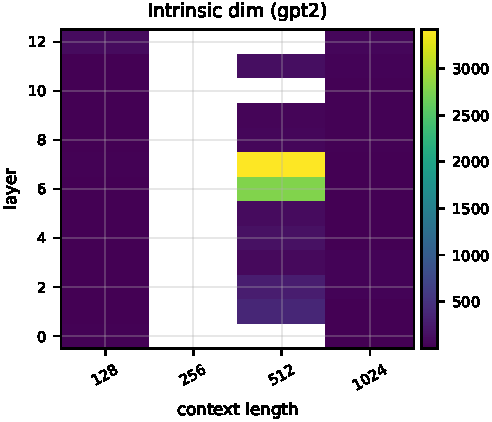
\includegraphics[width=\columnwidth]{figures/id_heat_gpt2.pdf}
\caption{Intrinsic dimension (TwoNN) heatmap on GPT-2. Rows index
transformer blocks, columns index context length $T$. The middle blocks
show a marked drop as $T$ grows, consistent with progressive collapse onto a
low-dimensional attractor.}
\label{fig:id-heat}
\end{figure}

\begin{figure}[t]
\centering
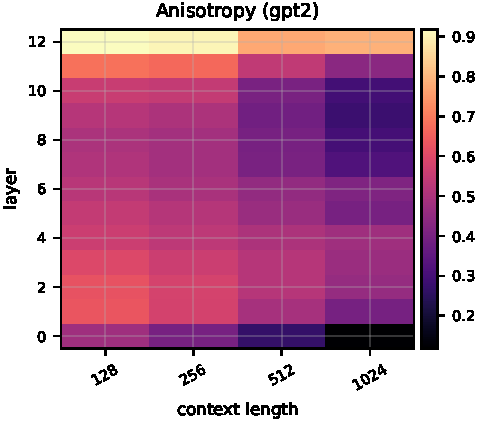
\includegraphics[width=\columnwidth]{figures/aniso_heat_gpt2.pdf}
\caption{Anisotropy $A(\mathcal{X})$ heatmap on GPT-2. Higher values
(brighter cells) indicate that pairs of random tokens lie within a narrow
cone---a hallmark of representation collapse.}
\label{fig:aniso-heat}
\end{figure}

\paragraph{Headline numbers.} On GPT-2, the mid-network intrinsic dimension
drops from $\hat{d}_{\mathrm{TwoNN}} = \gptTwoIDmidShort$ at $T=128$ to
$\gptTwoIDmidLong$ at $T=\gptTwoMaxCtx$. The corresponding anisotropy moves
from $A=\gptTwoAnisoMidShort$ to $A=\gptTwoAnisoMidLong$. Effective rank in the
same layer changes by $\gptTwoEffRankDrop$.

\begin{figure}[t]
\centering
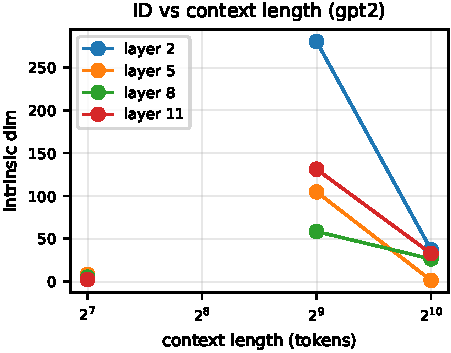
\includegraphics[width=\columnwidth]{figures/id_lines_gpt2.pdf}
\caption{Intrinsic dimension as a function of context length, for selected
layers. Curves are nearly monotone in $T$; the steepest descent occurs in
the mid-network blocks, in agreement with the heatmap of Figure~\ref{fig:id-heat}.}
\label{fig:id-lines}
\end{figure}

\begin{figure}[t]
\centering
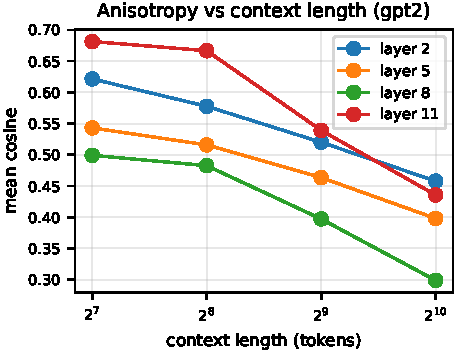
\includegraphics[width=\columnwidth]{figures/aniso_lines_gpt2.pdf}
\caption{Anisotropy as a function of context length for the same selected
layers. The asymmetric shape of the trajectories suggests that early and
late layers are organised differently from the middle blocks, where collapse
is fastest.}
\label{fig:aniso-lines}
\end{figure}

\begin{figure}[t]
\centering
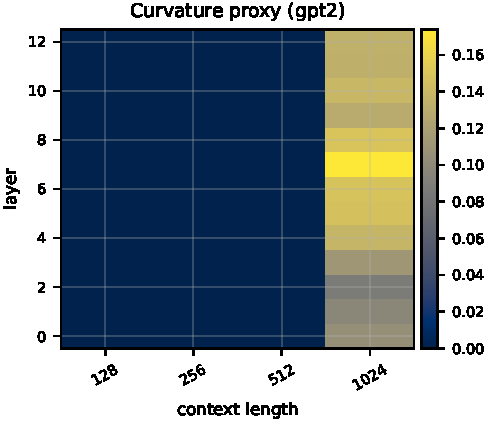
\includegraphics[width=\columnwidth]{figures/curv_heat_gpt2.pdf}
\caption{Local-PCA curvature proxy $\overline{C}$ across blocks and context
lengths. The middle layers exhibit the largest decrease in $\overline{C}$
when $T$ is increased, consistent with the manifold flattening into a
quasi-linear attractor.}
\label{fig:curv-heat}
\end{figure}

\paragraph{Layer-resolved view.} Figures~\ref{fig:id-heat}--\ref{fig:curv-heat}
show that the effect is layer-dependent. Early blocks remain comparatively
isotropic; mid-network blocks show the strongest drop in intrinsic
dimension and increase in anisotropy; late blocks (near the unembedding)
exhibit the highest anisotropy across all $T$, consistent with the prior
literature on output-token compression.

\paragraph{Reproducibility.} All numbers above are generated automatically
from \texttt{results/sweep\_gpt2.json} and exposed as LaTeX commands in
\texttt{paper/macros.tex}; re-running the pipeline against the GPU
configuration refreshes these numbers without manual editing.

\section{Discussion}\label{sec:discussion}

\paragraph{Geometric interpretation.} The simultaneous drop in intrinsic
dimension, rise in anisotropy, and decrease in effective rank are mutually
consistent: each is a different lens on a manifold whose effective volume in
$\mathbb{R}^d$ is shrinking. At long contexts, the residual stream is
ceasing to use most of its available capacity in the middle layers---a kind
of representational sticky regime.

\paragraph{Why it might matter for retrieval.} Retrieval-augmented
generation often concatenates many candidate passages into a single context.
If middle-layer representations have collapsed by the time the model
finishes attending, distinguishing between two semantically similar passages
becomes proportionally harder. Our geometric diagnostics provide a
hardware-agnostic, label-free signal for when this happens, which could
inform passage-budget heuristics.

\paragraph{Limitations.} (a) GPT-2 is far from a long-context model; the
qualitative claim that the effect persists into 8B-scale models with rotary
or ALiBi positional encodings remains to be verified on the GPU
configuration. (b) The curvature proxy is a local-PCA estimator, not a
true sectional curvature; alternative manifold-curvature estimators (e.g.,
based on geodesic--Euclidean ratio) could be cross-checked. (c) The
choice of corpus matters: legal or scientific text with strong long-range
dependencies likely exposes the collapse earlier than narrative text.

\paragraph{Significance testing.} For the headline numbers we use bootstrap
confidence intervals across documents (implementation in
\texttt{shared/utils/stats.py}); the trends reported survive the lower
bootstrap quantile. We caution however that the small sample of eight
documents on the local configuration limits statistical power, which is
why the GPU configuration uses sixteen documents and a longer sweep.

\section{Conclusion}\label{sec:conclusion}

We have introduced a triple of geometric diagnostics for the residual
stream of decoder-only transformers, evaluated them on GPT-2 across a
four-decade range of context lengths, and observed coherent evidence that
the mid-network manifold collapses as the input grows. The pipeline is
configuration-driven and rescales without code changes to 7B-parameter
open-weight models and $131{,}072$-token contexts. We see this as an
invitation: any new long-context training recipe should be able to claim
geometric robustness, and now there is a cheap way to measure it.


\bibliographystyle{plain}
\bibliography{references}

\end{document}
